%\title{Capstone Project Final Report}
%%%%%%%%%%%%%%%%%%%%%%%%%%%%%%%%%%%%%%%%%%%%%%%%%%%%%%%%%%%%%%%%%%%%%%%%%%%%%%%%
%2345678901234567890123456789012345678901234567890123456789012345678901234567890
%        1         2         3         4         5         6         7         8

\documentclass[letterpaper, 10 pt, conference]{ieeeconf}  % Comment this line out
                                                          % if you need a4paper
%\documentclass[a4paper, 10pt, conference]{ieeeconf}      % Use this line for a4
                                                          % paper
\maxdeadcycles=10000

\IEEEoverridecommandlockouts                              % This command is only
                                                          % needed if you want to
                                                          % use the \thanks command
\overrideIEEEmargins
% See the \addtolength command later in the file to balance the column lengths
% on the last page of the document

\usepackage{draftwatermark}
\SetWatermarkText{Draft}

\newcommand{\inputandref}[1]{\input{figs/#1.tex}\ref{fig:#1}}
\newcommand\Set[2]{\{\,#1\mid#2\,\}}

% The following packages can be found on http:\\www.ctan.org
\usepackage{graphicx} % for pdf, bitmapped graphics files
%\usepackage{epsfig} % for postscript graphics files
%\usepackage{mathptmx} % assumes new font selection scheme installed
%\usepackage{times} % assumes new font selection scheme installed
\usepackage{amsmath} % assumes amsmath package installed
\usepackage{amssymb}  % assumes amsmath package installed

\title{\LARGE \bf
Investigating the Relationship Between Plasticity and Evolvability in a Genetic Regulatory Network Model
}

\usepackage{etoolbox}
\patchcmd{\thebibliography}{\section*{\refname}}{}{}{}

\author{ \parbox{3 in}{\centering Matthew Andres Moreno
        \\
        University of Puget Sound\\
        4029 Wheelock Student Ctr., \\
        Tacoma, Washington\\
        {\tt\small mamoreno@pugetsound.edu}}
}

% \author{Huibert Kwakernaak$^{1}$ and Pradeep Misra$^{2}$% <-this % stops a space
% \thanks{*This work was not supported by any organization}% <-this % stops a space
% \thanks{$^{1}$H. Kwakernaak is with Faculty of Electrical Engineering, Mathematics and Computer Science,
%         University of Twente, 7500 AE Enschede, The Netherlands
%         {\tt\small h.kwakernaak at papercept.net}}%
% \thanks{$^{2}$P. Misra is with the Department of Electrical Engineering, Wright State University,
%         Dayton, OH 45435, USA
%         {\tt\small p.misra at ieee.org}}%
% }


\begin{document}



\maketitle
\thispagestyle{empty}
\pagestyle{empty}


%%%%%%%%%%%%%%%%%%%%%%%%%%%%%%%%%%%%%%%%%%%%%%%%%%%%%%%%%%%%%%%%%%%%%%%%%%%%%%%%
\begin{abstract}

Biological organisms are thought to possess traits that facilitate evolution.
The term evolvability was coined to describe this type of adaptation.
The question of evolvability has special practical relevance to computer science researchers engaged in longstanding efforts to harness evolution as an algorithm for automated design.
It is hoped that a more nuanced understanding of evolvability inspired by biological evolution will translate to more powerful digital evolution techniques.
To this end, the relationship between evolvability and environmental influence on the phenotype was investigated using digital experiments performed on a genetic regulatory model.
The phenotypic response of champion individuals evolved under regimes of direct plasticity, and indirect plasticity was assessed.
The model predicts that direct plasticity and indirect plasticity decrease and increase the frequency of silent mutations, respectively.


\end{abstract}


%%%%%%%%%%%%%%%%%%%%%%%%%%%%%%%%%%%%%%%%%%%%%%%%%%%%%%%%%%%%%%%%%%%%%%%%%%%%%%%%
\section{INTRODUCTION}

Evolvability is a principal concern to Evolutionary Algorithm researchers and evolutionary biologists alike. Although many competing definitions of evolvability exist in the literature, the general consensus is that evolvability stems from traits that facilitate the generation of viable heritable phenotypic variation \cite{Tarapore2015EvolvabilityBenchmarks}\footnote{This statement does not suggest that mutation is nonrandom, a controversial and widely discredited theory referred to biologists as adaptive mutation. Instead, it is predicated on the notion that the internal configuration of a biological system (i.e. the developmental process, modularity, degeneracy, etc.) constrains the outcomes of arbitrary perturbations to that system. It is hypothesized that biological organisms possess traits that influence the distribution of phenotypic effects of random mutation.} Breaking the concept down, evolvability stems from:
\begin{enumerate}
\item the amount of novel, heritable phenotypic variation among offspring, and
\item the degree to which heritable phenotypic variation among offspring is viable,\footnote{This can be thought of in terms of the frequency at which lethal or otherwise severely harmful mutational outcomes are observed.}
\end{enumerate}
The dependence of evolution on these capacities is straightforward. Without any heritable variation, evolution would have no raw material to select from and would stagnate. Without any viable variation, evolution would select against all novelty and again stagnate. Hence, systematic evolutionary change depends on the production of heritable, novel phenotypic variation, some of which must not be severely deleterious. We have established plausible traits that might facilitate evolution, but several important questions remain unanswered. How does evolvability manifest in biological organisms (i.e. what traits of biological organisms provide proximate explanations for the presence of viable heritable variation among offspring)? Why does evolvability manifest (i.e. what ultimate mechanistic forces endow biological organisms with traits that promote evolvability)? Addressing these two questions gives us a shot at tackling a third: how can evolvability be promoted in evolutionary algorithms?

It seems likely that evolvability stems from a large and diffuse set of contributing factors. The establishment -- or rejection -- of empirical causal links between theoretical complications of evolution and evolvability is a key research goal in the field; this type of inquiry will determine the complexity of a model necessary to account for evolution as observed in biological history and how complicated of a model is necessary to realize digital evolving systems with performance akin to their biological counterparts.

To this end, this research aims to investigate the relationship between environmental influence on the phenotype and evolvability.
It is hypothesized that organisms evolved under different regimes of environmental influence on the phenotype will exhibit different phenotypic responses to mutation.
To test this hypothesis, a series of digital experiments was performed with a genetic regulatory network model.
The gene regulatory network model is analogous to the transcription process of a biological cell.
In the model, a set of gene rules acts on a set of chemical concentrations, causing them to change over time.
The gene rules are influenced by the set of chemical concentrations they act on.
Rules may be activated and deactivated by the absence or presence of a chemical compound.
In the gene regulatory network model, the gene rules are said to represent the genotype.
Through the interpretation of the gene rules over simulated time, a phenotype --- the end set of chemical concentrations --- is developed.
In the context of the evolutionary process, the phenotype is evaluated to determine the fitness of a gene regulatory network.
The particular gene regulatory network model employed in this study was inspired by the model employed in \cite{Wilder2015ReconcilingEvolvability}.
This model was originally developed in \cite{Draghi2009TheModel}.

Gene regulatory networks were evolved under four regimes:
\begin{enumerate}
\item direct plasticity, where stochastic noise was introduced into the development process (Figure \inputandref{direct_plasticity_scheme}),
\item indirect plasticity, in which alternate environmental conditions indicate which of several alternate criteria phenotypes will be evaluated against (Figure \inputandref{indirect_plasticity_scheme}),
\item combined indirect-direct plasticity (Figure \inputandref{combined_plasticity_scheme}), and
\item control conditions (Figure \inputandref{control_scheme}).
\end{enumerate}
To assess the impact of these experimental conditions on evolvability, the response to mutation of champion individuals from populations evolved under each experimental condition was assessed.
Specifically, the frequency of three mutational outcomes was assessed:
\begin{enumerate}
\item silent mutation (mutation which is not phenotypically expressed),
\item lethal mutation (mutation which leads to a failure to develop a phenotype; in terms of the gene regulatory network model, this refers to mutations which cause the set of chemical concentrations to fail to converge after 500 applications of the set of gene rules),
\item non-lethal phenotypically expressed mutation (non-lethal mutation which leads to observable phenotypic effects).
\end{enumerate}


\section{BACKGROUND AND RELATED WORK}


\subsection{The Evolutionary Algorithm}


At the genesis of modern computing, the 1950s, researchers began to apply advancing computational capabilities to investigate and test models of biological evolution. Very quickly they realized the potential of virtual evolution to achieve other ends, setting into motion a line of research that has since blossomed into the field of evolutionary algorithms (EA) design. These algorithms, which use mechanics inspired by biological evolution to evolve novel solutions to a wide array of problems, share a generally consistent basic methodology. The process begins with a population of randomly generated solutions. In a generation-based loop, an elite subset of the population is selected for their fitness (their quality as a solution), subjected to random changes, and recombined with each other to form the next generation. The cycle repeats for as many iterations as desired, and fitness tends to increase with each iteration. Figure \inputandref{working_principle} provides a graphical overview of this process.

When discussing evolutionary algorithms (as well as their biological counterpart) an important distinction is drawn between phenotype and genotype. Phenotype refers to the characteristics of an individual that interact with its environment to determine its fitness. In biology, the physical form of an organism (i.e. its body) is the phenotype. In evolutionary algorithms, the phenotype refers to the characteristics of an individual that are evaluated during selection. Genotype refers to information that is used to determine the phenotype that is passed from generation to generation. In biology, a DNA sequence serves as the genotype. Although many different genotypic encodings are employed in evolutionary algorithms, the genotype ultimately boils down to a collection of digital information.

Researchers and engineers have widely demonstrated the ability of EA to attack labor-intensive optimization problems and to discover novel solutions beyond the reach of human ingenuity \cite{Poli2008AProgramming}. The intervening half century of EA research has seen diversification of the general evolutionary search process described above and diversification of the contents and format of candidate solutions. Today, evolutionary algorithms serve a dual purpose: a tool for biological inquiry and an algorithm for the automatic design of solutions to problems.

\subsection{Plasticity}

Plasticity refers to environmental influence on the phenotype. In biology, environmental and genetic influences, together, determine the phenotype. Environmental influences may alter the trajectory of the developmental process or may otherwise induce phenotype changes in response to environmental stimulus \cite{Fusco2010PhenotypicConcepts}. A conceptual distinction, which will be central to this investigation, can be drawn between direct and indirect plasticity. In the first, environmental influence is exerted directly on developmental or physiological processes. In the second, environmental signals prompt responses that are mediated by physiological or developmental systems; that is, cues from the environment are processed more like informational signals than coercive physical influence \cite{Fusco2010PhenotypicConcepts}. Although the distinction between a signal and coercive influence might appear nebulous at first blush, it has important implications to the design of the proposed experimental regime. At a fundamental level, successful direct plasticity entails \textit{resistance} to environmental influence on the phenotype while successful indirect plasticity entails strategic \textit{amplification} of environmental influence on the phenotype. Figures \inputandref{elephant_developmental_perturbation} and \inputandref{plant_developmental_perturbation} provide a cartoon illustration of this distinction. In Figure \ref{fig:elephant_developmental_perturbation} the cartoon elephant exhibits direct phenotypic plasticity, developing high-fitness phenotypic forms (which, in this example, appear nearly indistinguishable to a casual observer but in general need not be identical) despite variable environmental influence (i.e. diet, temperature, humidity, etc.). In Figure \ref{fig:plant_developmental_perturbation} the cartoon plant exhibits indirect plasticity, developing alternate phenotypic forms in response to variable environmental signals (i.e. light and shadow).

The exact role of phenotypic plasticity in evolution is an issue of active debate in the evolutionary biology community \cite{Pigliucci2008IsEvolvable}. However, several hypotheses describing how phenotypic plasticity might relate to evolution and evolvability have been put forward. Phenotypic plasticity might serve as a kind of local exploration of the phenotypic search space, allowing for the immediate expression of a phenotype with increased fitness and biasing the evolutionary search towards high-fitness regions of the search space \cite{Downing2012HeterochronousBaldwinism}. It is also thought that the homeostatic mechanisms that mediate an organism's interactions with its environment might promote robustness \cite{Moczek2011TheInnovation}. Researchers have suggested that phenotypic modularity might promote plasticity, especially in plants \cite{Schlichting1986ThePlants, DeKroon2005APlants}. Thus, selection for plasticity might promote modularity. In these ways, plasticity might promote useful variability.

Conditional expression of phenotypic traits through plasticity allows for relaxed selection on the genotypic locus determining those traits. Thus, significant genetic variation can accumulate at that locus in a population. In a process known as genetic accommodation, the environmental influence determining when rarely-expressed phenotypic traits are expressed can be diminished or erased through sensitizing mutation; what once was induced via environmental signals can become constitutive. Such processes have been observed experimentally via artificial selection \cite{Moczek2011TheInnovation}.

Finally, plasticity might play a role in concert with indirect genetic encodings, genetic encoding schemes without a direct one-to-one correspondence between genetic information and phenotypic information. Indirect encodings are biased towards phenotypic regularity, \cite{Clune2011OnRegularity} and plasticity might make available otherwise inaccessible phenotypic forms (i.e. providing a mechanism of irregular refinement of highly regular phenotypic structures generated from indirect encodings).


\section{METHODOLOGY}

The digital experimental framework used to investigate the relationship between plasticity and evolvability can be discussed in terms of three major components that compose it: the gene regulatory network model employed to perform the genotype-phenotype mapping, the criteria employed to assess phenotypic fitness, and the evolutionary algorithm employed to select on, mutate, and recombine genetic information.
These components will be described in Sections \ref{sec:grn}, \ref{sec:fitness}, and \ref{sec:ea}, respectively.
Then, a sketch of the approaches used to realize the digital experimental framework will be described in \ref{sec:implementation}.

\subsection{Gene Regulatory Network Model} \label{sec:grn}
The gene regulatory network model employed in this investigation was inspired by the approach reported in \cite{Wilder2015ReconcilingEvolvability} that was originally developed in \cite{Draghi2009TheModel}.
In this model employed by Wilder et al., the genotype is a directed graph with $k$ vertices where $k$ is the number of chemical products considered in the model.
Each node in the directed graph represents a single chemical product.
Experiments in \cite{Wilder2015ReconcilingEvolvability} used $k = 10$.
Connections between nodes represent gene rules.
Edge weights may only take on the values -1, 1, and 0.
Respectively, these edge weight values represent a inhibitory, excitatory, and neutral relationship between the source chemical product node and the destination chemical product node.
Thus, the genome may be represented by a $k \times k$ matrix $W$ where $W_{ij}$ represents the edge weight between transcriptional regulators $i$ and $j$.

An individual's phenotype is the pattern of chemical product concentrations induced by the action of gene rules on an initial state $S(0)$.
In this model, chemical concentrations are modeled as simple on/off states.
Thus, the set of chemical concentrations in the model at time step $n$, $S(n)$, can be represented as a simple bit vector.
To generate the phenotype, The following update rule is iteratively applied 500 times:
\begin{align*}
S_i(t+1) = 
\begin{cases}
1 & \text{if } \sum_{j=1}^{k} W_{ji}S_j(t) > 0 \\
0 & \text{otherwise.}
\end{cases}
\end{align*}
An individual is deemed viable if a fixed point is reached after 500 iterations (i.e. $S(500) = S(501)$).
If no fixed point is reached, the individual is deemed inviable and receives a fitness score smaller than those that would be assigned to all possible viable individuals.
Fitness scoring procedures are provided in detail in Section \ref{sec:fitness}.

Several adjustments were made to the model employed in \cite{Wilder2015ReconcilingEvolvability}.
Firstly, it was desired to work with a larger set of chemical concentrations, $k=98$,  than was employed in \cite{Wilder2015ReconcilingEvolvability}.
To avoid the $O(k^2)$ inflation of information stored in the genome, an alternate scheme was employed to represent the set of gene rules.
The set of gene rules was implemented as a set $\mathcal{S}$ of 392 individual if-then rules.
Each gene rule represents the action of one chemical product, the antecedent, on another, the patient.
As depicted in Figure \inputandref{grn_list}, the rule $R$ has three components: the index of a chemical antecedent $i$ denoted $R_a$, the index of a chemical patient $j$ denoted $R_p$, and a value $R_r$ describing the action of the antecedent on the patient.
As before, $R_r$ may take on the values -1, 1, and 0 to represent inhibitory, excitatory, and neutral relationships, respectively.
Thus, under this scheme each chemical concentration is updated according to the concentrations of the chemical products at the following timestep as follows:
\begin{align*}
S_i(t+1) = 
\begin{cases}
1 & \text{if } \sum_{R \in \mathcal{R}_i} R_r \times S_R(t) > 0 \\
0 & \text{otherwise.}
\end{cases}
\end{align*}
where $S_R(t) = S_j(t)$ with $j = R_a$ and $\mathcal{R}_i = \Set{R}{R \in \mathcal{S} \text{ and } R_p = i}$.
As before, to generate the phenotype this update rule is applied 500 times to an initial state $S(0)$ to generate the final state $S(500)$ and an individual is deemed inviable if $S(500) \neq S(501)$.
To enable sophisticated regulatory interactions in the network, it was desired to hide a portion of the chemical products from direct exposure in the phenotype.
Thus, the phenotype is defined as a subset of the set of chemical states $S(500)$.
In this case, the phenotype was defined as the end state of chemical products with indices 1 through 49, amounting to half of the chemical products acted on by the gene rules.

The experimental conditions of indirect and direct plasticity were realized by altering the initial set of chemical concentrations the gene regulatory network acts on (i.e. $S(0)$).
For each experiment, a set of chemical concentrations was generated at random with each initial chemical concentration having an equal probability of being set in the on or off state.
In control experiments, this set of chemical concentrations was employed directly as $S(0)$, remaining absolutely constant throughout each evolutionary run.
The control scheme is depicted in Figure \ref{fig:control_scheme}.
In direct plasticity experiments, a set of chemical concentrations is similarly generated.
However, at the outset of each individual development process, random changes are made to this initial set of chemical concentrations to form $S(0)$ for that individual development process. 
With probability $P$, each chemical concentration is randomly reassigned with equal probability to the on or off state.
The parameter $P$, which may range between 0 and 1, thus controls the severity with which environmental noise affects the developmental process.
The value $P = 0.2$ was used.
As in \cite{Reisinger2005TowardsEvolvability}, individual fitness was determined as the mean fitness score of several developmental runs.
In this case, 10 repeat evaluations were performed.
This direct plasticity scheme is depicted in Figure \ref{fig:direct_plasticity_scheme}.

In the indirect plasticity scheme, a distinct pair of sets of chemical concentrations are generated as in the control scheme.
A distinct pair of fitness criteria are also generated as discussed in Section \ref{sec:fitness}.
One fitness criteria, termed the primary objective, is paired with one set of chemical concentrations and the second fitness criteria, termed the secondary objective, is paired with the other set of chemical concentrations.
In this scheme, the development process performed twice, with $S(0)$ seeded once by each set of chemical concentrations. 
The phenotypes generated are evaluated according to the fitness criteria corresponding to the set of chemical concentrations used as $S(0)$.
Individual fitness is assessed as the mean fitness, weighted by a parameter $W$ representing the proportion of fitness determined by performance under the secondary environmental condition/objective pair.
The value $W = 0.2$ was used.
This indirect plasticity scheme is depicted in Figure \ref{fig:indirect_plasticity_scheme}. 

Finally, combined indirect and direct plasticity was realized by combining indirect and direct treatments of $S(0)$.
A weighted set of two environmental condition/objective pairings exposed to random perturbation of the initial state was employed.
The parameters $W = 0.33$ and $P = 0.2$ were used.
Five repeat evaluations were performed for each baseline initial condition evaluated.
The combined indirect and direct plasticity scheme is depicted in Figure \ref{fig:combined_plasticity_scheme}.

\subsection{Fitness criteria} \label{sec:fitness}
To study evolvability, it is desirable to avoid a direct correspondence between phenotypic distance and fitness.
Put more directly, it is desirable to work with fitness criteria where small phenotypic changes may on occasion result in significant fitness consequences and large phenotypic changes may on occasion result in slight fitness consequences.
Fitness consequence and magnitude of phenotypic change are necessarily correlated to some extent, but in a scheme without direct correspondence between these values, the effect of mutation in terms of the two major dimensions of evolvability, the generation of phenotypic novelty and phenotypic viability under mutation, can be teased apart to some degree \cite{Tarapore2015EvolvabilityBenchmarks}.
Thus, in the context of this research it was desired to avoid determining fitness via the hamming distance $d$ between an individual's gene expression profile and a target profile as was performed in \cite{Wilder2015ReconcilingEvolvability}.

Instead, fitness was measured by taking the phenotype as the initial state of a cellular automata simulation.
The fitness score is defined as the value of certain metric assessed from the set of states generated by the cellular automata simulation  (discussed below).
It was determined that such a scheme would provide the desired indirect relationship between fitness consequence and magnitude of phenotypic effect of mutation.
In this case, the set of cellular automata rules known as Conway's game of life was employed \cite{Conway1970TheLife}.
The phenotype generated via the gene regulatory network, a set of on/off states, were arranged into a two dimensional grid.
In this case, the grid had dimensions $7 \times 7$.
The series of grid states $G = \{g_1, g_2, g_3 \ldots g_30\}$ resulting from 30 sequential applications of Conway's game of life rules were recorded.
A cutoff parameter $1 < C < 30$ defines a particular fitness criteria.
Fitness is assessed from the ratios of live cells (grid tiles in the active state) to dead cells (grid tiles in the inactive state) observed in the grid states preceding and following the cutoff time coordinate.
Fitness is thus calculated as,
\begin{align*}
\frac{\sum_{i=1}^{n<C} L(g_i)}{C} - \frac{\sum_{i=C}^{n<30} L(g_i)}{30 - C}
\end{align*}
where $L(g)$ represents a count of the live cells present in Conway grid state $g$.
Under this scheme, a phenotype from which a high density of live cells is observed prior to the cutoff time coordinate and a low density of live cells is observed following the cutoff time coordinate will enjoy high fitness.
Note that the fitness is normalized to fall strictly in the range $[-1, 1]$.
Thus, with a fitness value of $-1$ assigned to non-convergent individuals, convergent individuals will enjoy a selective advantage against non-convergent individuals.
The ability to readily define alternate fitness criteria is essential to this research (i.e. to experimentally realize indirect plasticity).
Adjustment of the cutoff parameter $C$ provides an avenue to this end.

\subsection{Evolutionary Algorithm} \label{sec:ea}
Selection, mutation, and recombination of genetic material was performed with the Distributed Evolutionary Algorithms in Python (DEAP) framework \cite{Fortin2012DEAP:Easy}.
A population size of 50 individuals was employed.
At the outset of each generation, each available space in the population was filled by tournament-style selection of the most fit individual among a randomly selected group of five individuals.
This procedure was performed using DEAP's \texttt{selTournament} tool.
Exchange of genetic material via two-point crossover was then performed among members of the new generation with DEAP's \texttt{cxTwoPoint} tool with crossover between each pairing occurring with probability 0.5.
Finally, with probability 0.2, mutation was applied to each member of the new generation.
If an individual was selected for mutation, the number of point mutations the individual experienced was drawn from a binomial distribution with $n=392$, the number of rules present in the genome, and $p=0.1$.
For each point mutation, a rule was selected at random from the set of 392 rules that compose the genome.
Mutation was performed by selecting a random rule from an individual's genome, selecting a component of the rule at random with equal probability (i.e. $R_a$, $R_r$, or $R_p$), and reassigning the rule component to a selection drawn with equal probability from the set of valid values for that component.

\subsection{Implementation} \label{sec:implementation}
The digital experiments performed required significant computational power, especially in light of the replicate trials necessary to establish statistical significance.
Fortunately, evolutionary algorithms are amenable to massive parallelization.
Fitness evaluations of individuals in a population can be readily performed in parallel.
In order to exploit parallel processing power, experiments were performed on remote clusters.
Even with this parallel processing power, performing replicate experiments required the better part of a day. 
The software with which simulations were performed was structured as a Python package.
This software package was written and tested on a local machine, then installed on a remote cluster.
This development scheme, which strictly separated code implementing the model from code written to perform experiments with the model, allowed the model to be kept under strict version control.
Computational tests were performed and recorded using Jupyter notebooks hosted on the remote cluster.
These notebooks provided a convenient mechanism to catalog and annotate code written to perform experiments and results from those experiments, both in the form of printed console output and graphical output generated via Pyplot.
Data from computational experiments was saved on the remote clusters using the Pickle Object Serialization tool.
Jupyter notebooks, which are served as HTML documents, are readily accessible from a local machine.



\section{RESULTS}

Results from experiments investigating the relationship between direct, indirect, and combined plasticity are reported in Sections \ref{sec:direct_result}, \ref{sec:indirect_result}, and \ref{sec:combined_result}.
To summarize, the emergence of gene regulatory networks exhibiting direct and indirect plasticity was observed in evolutionary trials where environmental influence on the phenotype exerted selective pressure for these traits.
Champion gene regulatory networks from evolutionary trials selecting for direct plasticity exhibited a higher incidence of silent mutation compared to champion gene regulatory networks evolved in control trials.
Champion gene regulatory networks from evolutionary trials selecting for indirect plasticity exhibited a higher incidence of phenotypically-expressed mutation and a lower incidence of silent mutation compared to champion gene regulatory networks evolved in control trials.
Both of these experimental treatments appear to leave the rate of lethal mutation unaffected.
Champion gene regulatory networks from evolutionary trials selecting for both indirect and direct plasticity exhibited a higher incidence of phenotypically expressed mutation.

\subsection{Direct Plasticity} \label{sec:direct_result}
The capacity of the gene regulatory networks modeled herein to exhibit direct plasticity --- the ability to consistently develop high-fitness phenotypes despite environmental noise --- was confirmed by comparison of the fitness achieved by champion individuals under exposure to environmental noise to a control group.
It was confirmed that champion individuals from the direct plasticity regime achieved fitness comparable to individuals evolved under a control regime.
Thus, it was concluded that the gene regulatory networks evolved were capable of coherent function despite some environmental noise.

Figure \ref{fig:es_direct} compares the evolvability signature of champion individuals evolved with and without environmental perturbation.
\begin{figure}
    \centering
    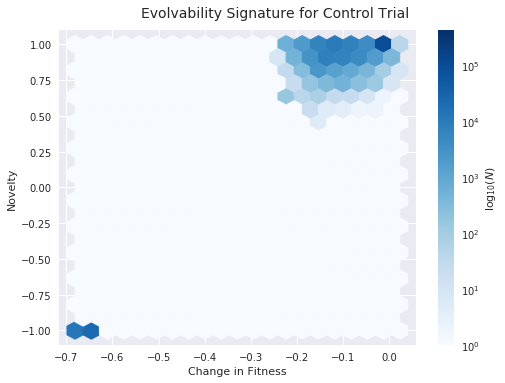
\includegraphics[width=0.5\textwidth]{img/es_p0} \\
    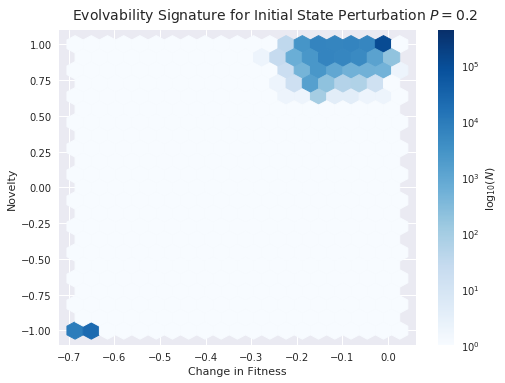
\includegraphics[width=0.5\textwidth]{img/es_p0_2}
\caption{Evolvability signatures of champion evolved without initial plasticity ($P = 0$) (top) and with initial plasticity ($P=0.2$). Figure after \cite{Tarapore2015EvolvabilityBenchmarks}.}
    \label{fig:es_direct}
\end{figure}
The evolvability signature co-visualizes the phenotypic and fitness outcomes of mutation.
Phenotypic novelty resulting from mutation, measured via the hamming distance between the phenotype expressed prior to and following mutation, is plotted on the $y$ axis.
Relative fitness of the phenotypes expressed prior to and following mutation is plotted on the $x$ axis.
The darkness of each tile represents the frequency of mutational outcomes that fall into that bin.
Silent mutations occur at the top right of the diagram, at the juncture of 0 novelty and 0 fitness consequence.
Lethal mutations are clustered at the bottom left of the evolvability signature.
Compared to the control evolvability signature, an overall reduction in the frequency of mutation with significant phenotypic and/or fitness consequences is observed under the direct plasticity regime.

This observation is accounted for in Figure \ref{fig:mutation_type_direct}, which compares the relative frequency with which silent, lethal, and phenotypically-expressed outcomes are observed from champion individuals evolved under the control and direct plasticity regimes.
\begin{figure}
    \centering
    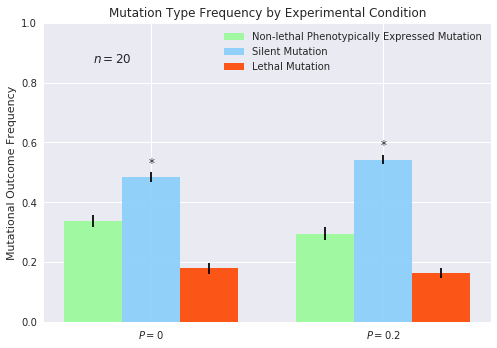
\includegraphics[width=0.5\textwidth]{img/mutation_type_direct}
  	\caption{Comparison of mutational outcome frequencies for champions evolved with and without initial state perturbation.}
    \label{fig:mutation_type_direct}
\end{figure}
A statistically significant increase in the incidence of silent mutation is observed under the direct plasticity regime.
This increase in the incidence of silent mutation appears to correspond to slight decreases in both the rates of lethal mutation and phenotypically expressed non-lethal mutation.

\subsection{Indirect Plasticity} \label{sec:indirect_result}
The capacity of the gene regulatory networks modeled herein to exhibit indirect plasticity --- the ability to simultaneously achieve high-fitness to a set of two of environmental condition/objective pairings --- was confirmed by comparison of the fitness scores for each environmental condition/objective pairing between champion individuals evolved with fitness determined exclusively via the primary condition/objective pairing and those evolved with fitness determined by both primary condition/objective pairings.
As expected, it was found that individuals exposed to the secondary condition/objective paring significantly outperformed individuals that were not with respect to that condition/objective pairing.
Champion individuals evolved exclusively to satisfy the primary condition/objective pairing exhibited statistically significant greater performance under the primary condition/objective pairing compared to individuals evolved to satisfy both condition/objective parings.
Nevertheless, the performance of champion individuals evolved to satisfy both condition/objective pairings at the primary condition/objective pairing was roughly comparable to that of champion individuals evolved exclusively to satisfy the primary condition/objective pairing; individuals evolved to satisfy both condition/objective pairings exhibited an obvious capacity to satisfy the primary condition/objective pairing.
These results are presented in Figure \ref{fig:primary_secondary_performance}.
It was concluded that the gene regulatory networks evolved in this model were capable of exhibiting indirect plasticity, simultaneously providing good performance on multiple condition/objective pairings.

\begin{figure}
    \centering
    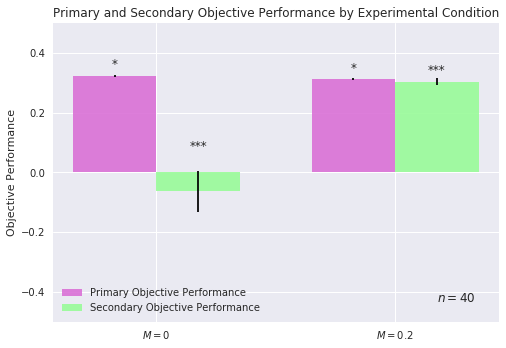
\includegraphics[width=0.5\textwidth]{img/primary_secondary_performance}
  	\caption{Comparison of objective performances of champions evolved with only primary condition/objective pair versus with both primary and secondary condition/objective pairs.}
    \label{fig:primary_secondary_performance}
\end{figure}

Figure \ref{fig:ev_indirect} compares evolvability visualizations of champion individuals evolved under control conditions, where selection took place exclusively for the primary condition/objective pairing, to individuals evolved to simultaneously satisfy both condition/objective pairings.
These visualizations were generated by measuring performance exclusively in terms of the primary condition/objective pairing.
These visualizations are comparable to the evolvability signatures provided in Figure \ref{fig:es_direct}, but track absolute fitness on the $x$ axis in lieu of relative fitness.
This change was made to ensure a clear comparison of the outcomes of mutation between champion individuals evolved exclusively under the control conditions, which enjoy slightly greater fitness in terms of the primary condition/objective pairing, and champion individuals evolved to simultaneously satisfy both condition/objective pairings.
A lower right hand region is outlined in red on these visualizations.
This region, the exact bounds of which were chosen arbitrarily, represents mutational outcomes in which mild fitness consequences are observed despite nontrivial phenotypic novelty.
Such mutational outcomes are desirable in terms of evolvability.
Preliminary analysis suggests that, despite overall relatively lower fitness of champion individuals, champion individuals evolved under an indirect plasticity regime more frequently generate mutational outcomes that fall into this region. 
More sophisticated statistical investigation would be necessary to confirm this finding.

\begin{figure}
    \centering
    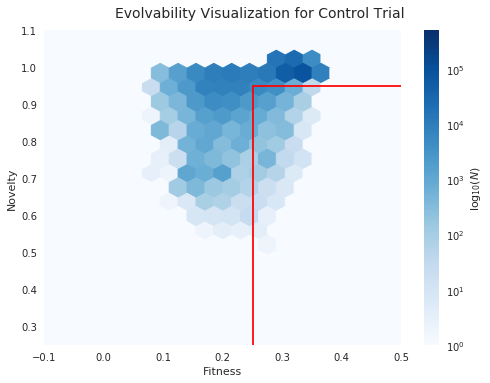
\includegraphics[width=0.5\textwidth]{img/ev_w0_target} \\
     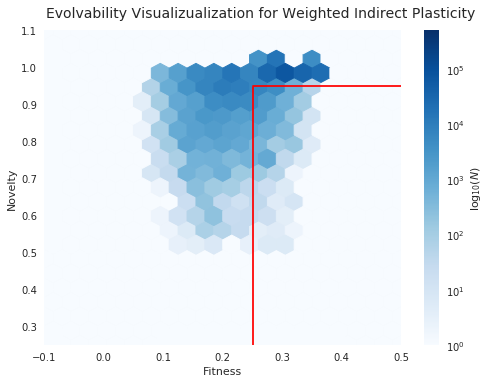
\includegraphics[width=0.5\textwidth]{img/ev_w0_2_target}
  	\caption{Evolvability visualization of champions evolved with only a primary condition/objective pair (top) and champions evolved with primary and secondary condition/objective pairs (bottom).}
    \label{fig:ev_indirect}
\end{figure}

Figure \ref{fig:mutation_type_indirect} compares the relative frequency with which silent, lethal, and phenotypically-expressed outcomes are observed from champion individuals evolved under control and indirect plasticity regimes.
It was found that evolution under the indirect plasticity regime induces a statistically-significant decrease in the frequency of silent mutation and a corresponding statistically-significant increase in the frequency of phenotypically-expressed non-lethal mutation.
The frequency of lethal mutation was not obviously affected.

\begin{figure}
    \centering
    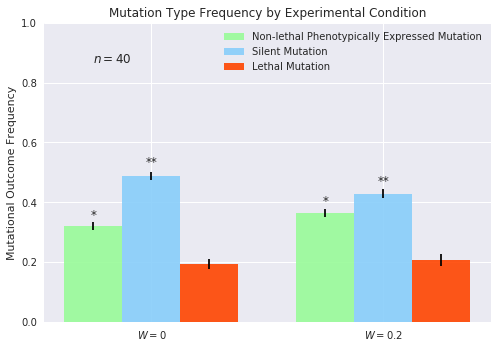
\includegraphics[width=0.5\textwidth]{img/mutation_type_indirect}
  	\caption{Comparison of mutational outcome frequencies for champions evolved with only primary condition/objective pair versus with both primary and secondary condition/objective pairs.}
    \label{fig:mutation_type_indirect}
\end{figure}

\subsection{Combined Plasticity} \label{sec:combined_result}
Similar to validation of the capacity of evolved gene regulatory networks to exhibit direct and indirect plasticity (reported in Sections \ref{sec:direct_result} and \ref{sec:indirect_result}), the capacity of evolved gene regulatory networks to exhibit both direct and indirect plasticity simultaneously was confirmed.
Specifically, it was found that champion individuals evolved under the combined plasticity regime exhibited comparable fitness relative to champion individuals evolved under the control regime in terms of the primary condition/objective pairing.
Figure \ref{fig:mutation_type_indirect} compares the relative frequency with which silent, lethal, and phenotypically-expressed outcomes are observed from champion individuals evolved under the control and combined plasticity regimes.
It was found that evolution under the combined plasticity regime induces a statistically-significant decrease in the frequency of silent mutation and a corresponding statistically-significant increase in the frequency of which phenotypically-expressed non-lethal mutation is observed.
Although not strong enough to merit statistical significance, this change in the frequency of phenotypically-expressed non-lethal mutation appeared to be accompanied by a corresponding decrease in both the frequency of silent mutation and the frequency of lethal mutation.

\begin{figure}
    \centering
    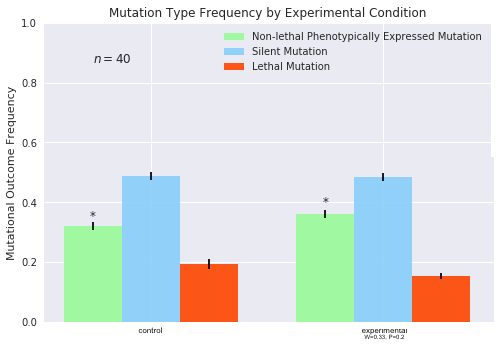
\includegraphics[width=0.5\textwidth]{img/mutation_type_combined}
  	\caption{Comparison of mutational outcome frequencies for champions evolved with only primary condition/objective pair and no initial state perturbation versus with both primary and secondary condition/objective pairs and initial state perturbation.}
    \label{fig:mutation_type_combined}
\end{figure}

\section{DISCUSSION}

Experiments reported in Section ref{sec:results} confirm that environmental influence on the phenotype affects the outcomes of mutation of champion individuals.
These experiments therefore evidence a relationship between phenotypic plasticity and evolvability.
This finding opens questions about the exact nature of this relationship and, in particular, how the relationship mechanistically operates.

Evolvability is commonly understood in terms of internal structural configuration of an evolving system.
Work performed by Draghi and Wagner investigating evolvability in a highly abstract, simplified evolutionary model illustrates the connection between internal structural configuration and evolvability \cite{Draghi2008EVOLUTIONMODEL}.
The phenotype in their model is a coordinate in two-dimensional space. 
Genotypically, individuals are represented as a pair of vectors.
Individuals for which a near right angle exists between their pair of genotypic vectors are considered more evolvable compared to individuals for which these two vectors are near parallel.
The near-perpendicular internal configuration allows for a greater range of phenotypic outcomes (i.e. points in two-dimensional space) to be realized by mutations that affect vector length.

Consideration of how internal structural characteristics might bridge the gap between environmental influence on the phenotype and evolvabilitiy can be brought explicitly into terms of the gene regulatory network model explored in this paper.
It is hypothesized that environmental noise induced selection for internal structural configurations capable of mitigating that noise which, in turn, caused an increase in the frequency of silent mutation.
The presence of alternate phenotypic targets in the context of multiple condition/objective pairings is hypothesized to have induced selection for internal structural configurations capable of facilitating developmental path switching which, in turn, caused a decrease in the frequency of silent mutation.
The exact nature of these internal structural configurations remains an open question.
The internal configuration of individuals --- the gene regulatory network rules through which the phenotype is generated --- can be represented as a directed graph.
Preliminary analysis of various graph metrics --- the overall occurrence of different types of connections (i.e. inhibitory, excitatory, and neutral) between nodes, the distribution of connection counts between each node, the number of isolated subgraphs present etc. --- did not reveal any obvious differences in the graph structures characteristic of champions evolved under different experimental regimes.
A more comprehensive effort to characterize the graph structure of champions evolved under different experimental regimes, in particular to visualize the gene regulatory graphs of individual champion solutions as well as the aggregate structural characteristics of a set of champion solutions evolved under the same experimental regime, might shed light on internal structural configurations that promote direct plasticity and indirect plasticity.

A key question to address is how the internal structural configurations that promote direct and indirect plasticity relate to one another.
Direct and indirect plasticity may stem from vastly different aspects of internal structural configuration, identical aspects of internal structure configuration (likely in opposite polarities), or some intermediate between the two.
The frequency of mutational outcomes, reported in Figure \ref{fig:mutation_type_combined}, shed some light on this question.
Simultaneous selection for direct and indirect plasticity does not seem to result in a simple ``canceling out'' of the evolvability characteristics exhibited by champion individuals selected for direct and indirect plasticity in isolation.
Instead, there is an increase of the rate at which phenotypically-expressed non-lethal mutation is observed while the rate of silent mutation is not strongly affected.
This result may suggest that direct and indirect plasticity stem from different aspects of internal structural configuration. 

\section{FUTURE WORK}

As many exciting scientific inquiries do, this investigation raises as many questions as it answers.
Work remains to be done, both with this particular computational model of evolution and more broadly.
Most pressingly, it is hoped that continued investigation will shed light on internal structural characteristics that support direct and indirect plasticity.
It would also be worthwhile to attempt to demonstrate a situation in which search with plasticity outperforms search without in terms of the absolute fitness of champion solutions evolved.
More broadly, it would be fruitful to perform similar experiments with a more directly biologically-inspired model or even \textit{in vivo}.

\section{CONCLUSION}

The relationship between evolvability and environmental influence on the phenotype was investigated using digital experiments performed on a genetic regulatory model.
The capacity of the model to accommodate the emergence of direct, indirect, and combined plasticity in evolved genetic regulatory networks was confirmed.
The phenotypic response of champion individuals evolved under regimes of direct plasticity and indirect plasticity was assessed.
The model predicts that direct plasticity and indirect plasticity decrease and increase the frequency of silent mutations, respectively.
The model also predicts that combined plasticity induces an increase in the frequency of phenotypically-expressed non-lethal mutation without having a noticeable effect on the observed frequency of silent mutation.

These experimental results confirm the existence of a relationship between phenotypic plasticity and evolvability.
It is hypothesized that this relationship is mediated by internal structural characteristics of the evolved gene regulatory networks.
Specifically, it is postulated that environmental influence on the phenotype induces selection for certain internal characteristics that support direct and/or indirect plasticity which, in turn, affect the outcome of mutation.
The exact nature of internal structural characteristics that support direct and indirect plasticity remains unknown.
Analysis of the outcome of mutation of champion individuals evolved under a combined plasticity regime in comparison to individuals evolved under just a direct plasticity regime and just an indirect plasticity regime suggests that direct and indirect plasticity stem from different aspects of internal structural configuration. 
Further work is called for to pin down a structural characterization of the internal characteristics that support direct and indirect plasticity in order to investigate the hypothesized nature of the relationship between evolvability and phenotypic plasticity.



\addtolength{\textheight}{-12cm}   % This command serves to balance the column lengths
                                  % on the last page of the document manually. It shortens
                                  % the textheight of the last page by a suitable amount.
                                  % This command does not take effect until the next page
                                  % so it should come on the page before the last. Make
                                  % sure that you do not shorten the textheight too much.

%%%%%%%%%%%%%%%%%%%%%%%%%%%%%%%%%%%%%%%%%%%%%%%%%%%%%%%%%%%%%%%%%%%%%%%%%%%%%%%%



%%%%%%%%%%%%%%%%%%%%%%%%%%%%%%%%%%%%%%%%%%%%%%%%%%%%%%%%%%%%%%%%%%%%%%%%%%%%%%%%

\section*{ACKNOWLEDGEMENT}
The author would like to acknowledge the authors of the Distributed Evolutionary Algorithms in Python package, upon which much of the computational work performed in this investigation was based, and Professor David Chiu of the University of Puget Sound for his generous contribution of cluster compute time.


%%%%%%%%%%%%%%%%%%%%%%%%%%%%%%%%%%%%%%%%%%%%%%%%%%%%%%%%%%%%%%%%%%%%%%%%%%%%%%%%



\bibliography{Mendeley}
\bibliographystyle{ieeetr}



\end{document}
